\section{Part A}%
\label{a}


\begin{figure}[H]
	\centering
	\captionsetup{justification=centering}
	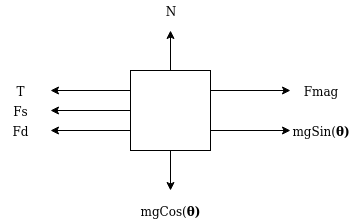
\includegraphics[width=0.8\linewidth]{imgs/FBD.png}
	\caption{Free-body diagram of forces acting upon the ball}%
	\label{fig:14}
\end{figure}

Forces on x-axis : \\
\[
Fmag + mg \sin (\theta ) - T - Fs - Fd = m \ddot x\label{eq:1} \tag{\ding{1}}
\]

$Fs = k(x-d)$\\
$Fd = b\dot x$


Forces on y-axis: \\
$N - mg\cos(\theta) = 0$  - (2)

Moment of inertia, i = $2/5mr^2$

Torque $M = -Tr$          (-Ve as rotating clockwise)

$I\ddot \theta = -Tr \rightarrow  1/2 mr^{\cancel{2}} \ddot\theta = -T\cancel{r}$

$T = -1/2 mr\ddot\theta$ 

By 'Pizza slice theorem', $\ddot x = \ddot \theta r$

Therefore, 
$T = 1/2 m \ddot x$ \\

Finding magnet force, Fmag

$Fmag = C \frac{I^2}{R^2}$    -  (2)

Applying Kirchoffs Voltage Law on loop,\\
$V = IR + \dot I C$

$$\int V dy = IR \int 1\cdot dy + C \int \frac{di}{dy} dy$

$Vy = IRy + LI$

$Vy = I(Ry + L)$

$I = \frac{Vy}{Ry+L}$ -   (3)

Substituting (3) into (2)

$Fmag = \frac{CV^2y^2}{(Ry + L)^2 y^2} = \frac{C}{(Ry+L)^2}V^2$ - (4)

Substituting (4) into (1)

$$\frac{CV^2}{(Ry+L)^2} + mg\sin(\theta) -k(x-d) - b\dot x = \frac{1}{2}m\ddot x $

\textbf{A2}  \\

    $x_{1} = x$
    
   $x_{2} = \dot x_{1} = \dot x$
   
    $\dot x_{2} = \ddot x$
    
    

    \underline{x}=
\left\{\begin{matrix}
\dot x = x_{2}
\\ 
\frac{2CV^2}{(Ry+L)^2m} + 2g\sin(\theta) - \frac{2k}{m}(x_{1}-d) - \frac{2b}{m} x_{2} = \dot x_{2}
\end{matrix}\right.

\textbf{A3}  \\

$\dot x = f(x, V)$, a pair $(x^eq , V^eq)$ is an equilibrium point if $f(x^eq, V^eq) = 0$
\\


at equilibrium, $d = 0$

    \underline{x^{eq}}=
\left\{\begin{matrix}
x_{2}^{eq} = 0
\\ 
\frac{2CV^2}{(Ry+L)^2m} + 2g\sin(\theta) - \frac{2k}{m}(x_{1}^{eq}-0) - \frac{2b}{m} x_{2}^{eq} = 0
\end{matrix}\right.
\\

\textbf{A4}


\pagebreak
